%Compare to phones!
Compared to smartphones one of the biggest advantages of Google Glass is the fact that Google Glass is a HMD. With a smartphone the user needs to either hold the smartphone in either one or both hands, or alternatively put the smartphone on a table. In other words can Google Glass offer a hands-free experience that smartphones cannot.

Another advantage of Google Glass compared to smartphones also comes from the fact that Google Glass is an HMD. The user does not need to look away in order to see what is currently being displayed. Google Glass does not distract from what the user is currently doing as much as a smartphone where the user needs to either look away or hold up the smartphone in from of their eyes.

However, smartphones does give the user a bit more control. The control comes from the fact that smartphones supports multi-touch, which Google Glass does not. On a smartphone users may also touch directly on the screen, in contrast to Google Glass where the touchpad sits on the right hand side of the user. Smartphones also have a larger touch area than Google Glass.

The smartphone screen size has been increasing ever since the iPhone first launched in 2007~\cite{iphoneWiki}, as seen in Figure~\ref{smartphoneSizeChart2}. Looking at currently available smartphones, in Figure~\ref{smartphoneSizeChart}, the increase in screen size does is set to continue as the average screen size is approaching five inches. In terms of comparison with Google Glass the increase in screen size entails that more information could be displayed on a smartphone than on Google Glass.

%\url{https://developer.android.com/design/index.html}\\
%\url{https://developer.android.com/design/get-started/principles.html}
	\begin{figure}[ht!]
		\centering
		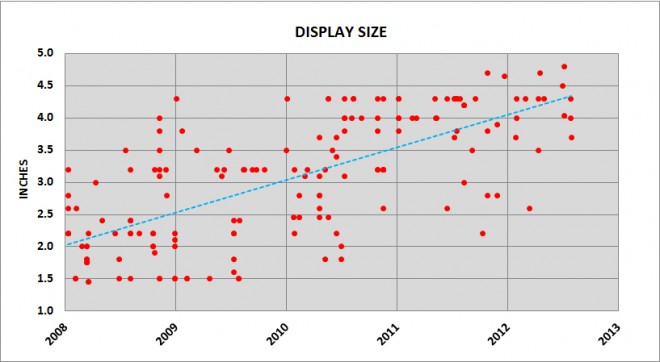
\includegraphics[width=110mm]{images/smartphoneSize2}
		\caption{Smartphone screens have been increasing in size for several years~\cite{smartphoneSizeChart2}.}
		\label{smartphoneSizeChart2}
	\end{figure}
	%http://www.pcworld.com/article/2455169/why-smartphone-screens-are-getting-bigger-specs-reveal-a-surprising-story.html
	
	
	\begin{figure}[ht!]
		\centering
		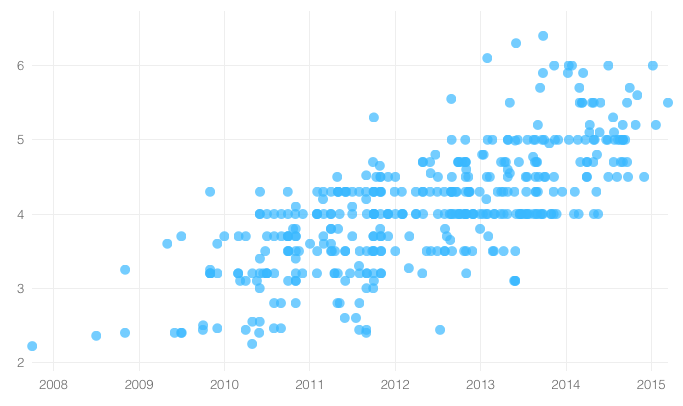
\includegraphics[width=110mm]{images/smartphoneSize}
		\caption{Screen sizes of the most popular, currently available smartphones~\cite{smartphoneSizeChart}.}
		\label{smartphoneSizeChart}
	\end{figure}

However, one of the biggest differences between smartphones and Google Glass is the plural, smartphone\textbf{s}. There are several smartphone brands competing on the market, each offering several models. Google Glass is simply Google Glass, one product. As seen in section~\ref{subsec:similarproducts} Google Glass does face competitors that have approached HMDs differently, and as HMDs increase in popularity there is potential for an even wider offering of models and screen sizes.

%\url{https://developer.android.com/design/index.html}\\
%\url{https://developer.android.com/design/get-started/principles.html}

	%http://www.pcworld.com/article/2455169/why-smartphone-screens-are-getting-bigger-specs-reveal-a-surprising-story.html

% Color schemes
% pre defined layouts
% pre defined typography (fonts)





